\chapter{Fish Tank Suite}
\label{fts:chapter}
In diesem Kapitel wird folgende Frage beantwortet: \textit{''Wie würde eine Software aussehen, die für den Einsatz in einem realen Szenario geeignet ist?''}.\\

Bei der Fish Tank Suite handelt es sich um eine Software, die aus den Erkenntnissen der Analyse und Prototypen hervorging. Diese Software soll eine praxistaugliche Lösung für die Probleme der Ausgabenstellung darstellen.

\section{Akteure}
\begin{table}[H]
    \centering
    \begin{tabularx}{\textwidth}{| l | X |}
        \hline
        \textbf{Rolle}     & \textbf{Beschreibung}    \\ \hline
        \textbf{Auftraggeber}  & Der Auftraggeber möchte einen lauffähigen Prototypen, der die Machbarkeit des Projekts beweist.  \\ \hline
        \textbf{Entwickler} & Der Entwickler ist für die Entwicklung der Software zuständig.   \\ \hline
        \textbf{IT-Security Engineer} & Anwender der Software.   \\ \hline
    \end{tabularx}
    \caption{Fish Tank Suite: Akteure}
\end{table}

\section{User Stories}
\subsection{Sprint 3}
% Sprint 3 -> RC1
\begin{epic}{Epic 3: Release Candidate 1}
  Ende Sprint soll ein erster Release Candidate erstellt sein.
\end{epic}

\begin{story}{Story 3.1:  Chunked Data}
  Als Entwickler will ich chunked Data speichern können.
  \tcblower
  \textbf{Akzeptanzkriterien}
  \begin{itemize}
  	\item Ganze Requests und Responses können gespeichert werden.
  	\item Begin und End of Data von \gls{icap} werden nicht mehr geloggt.
  \end{itemize}
\end{story}

\begin{story}{Story 3.2:  Log Daten}
  Als Entwickler will ich eine performante Analyse der Log Daten.
  \tcblower
  \textbf{Akzeptanzkriterien}
  \begin{itemize}
  	\item Das Durchsuchen der Elasticsearch wurde im Vergleich zum Prototyp effizienter.
  	\item Das Loggen von Daten wurde effizienter.
  \end{itemize}
\end{story}

\begin{story}{Story 3.3:  Verschlüsselter Payload}
  Als Security Engineer will ich verschlüsselten Payload analysieren können.
  \tcblower
  \textbf{Akzeptanzkriterien}
  \begin{itemize}
  	\item Payload Entschlüsselung möglich.
  	\item Verschlüsselter Payload wird geloggt.
  \end{itemize}
\end{story}

\begin{story}{Story 3.4:  Verschlüsselter Payload erkennen}
  Als Entwickler will ich erkennen, ob der Payload verschlüsselt ist.
  \tcblower
  \textbf{Akzeptanzkriterien}
  \begin{itemize}
  	\item Anhand von Keywords möglich zu testen, ob entschlüsselt.
  \end{itemize}
\end{story}

\begin{story}{Story 3.5: Fake \gls{cc}}
  Als Entwickler will ich einen Fake \gls{cc} zum Testen.
  \tcblower
  \textbf{Akzeptanzkriterien}
  \begin{itemize}
  	\item Requests können weitergeleitet werden.
  	\item Responses, die bösartige Malware beinhalten, können nicht weiter senden.
  \end{itemize}
\end{story}

\begin{story}{Story 3.6:  Campaign}
  Als Security Engineer will ich eine Campaign definieren.
  \tcblower
  \textbf{Akzeptanzkriterien}
  \begin{itemize}
  	\item Campaign JSON mit möglichen Optionen definiert.
  \end{itemize}
\end{story}


\begin{story}{Story 3.7:  Projektdokumentation}
  Als Entwickler will ich eine aktuelle Dokumentation.
    \tcblower
  \textbf{Akzeptanzkriterien}
  \begin{itemize}
  	\item Dokumentation wird laufend erweitert.
  \end{itemize}
\end{story}

\subsection{Sprint 4}

\begin{epic}{Epic 4: Release Candidate 2}
  Ende Sprint soll ein zweiter Release Candidate erstellt sein.
\end{epic}


\begin{story}{Story 4.1:  Projektdokumentation}
  Als Entwickler will ich eine aktuelle Dokumentation.
  \tcblower
  \textbf{Akzeptanzkriterien}
  \begin{itemize}
  	\item Dokumentation wird laufend erweitert.
  \end{itemize}
\end{story}

\begin{story}{Story 4.2:  Zentrale Verwaltung}
  Als Security Engineer will ich mehrere Systeme über einen zentralen Punkt verwalten.
  \tcblower
  \textbf{Akzeptanzkriterien}
  \begin{itemize}
  	\item Campaign an zentralem Punkt gespeichert.
  	\item Änderungen für andere Systeme werden übernommen.
  \end{itemize}
\end{story}


\begin{story}{Story 4.3:  \gls{aes128} Payload}
  Als Auftraggeber will ich Payload mit \gls{aes128} entschlüsseln können.
  \tcblower
  \textbf{Akzeptanzkriterien}
  \begin{itemize}
  	\item \gls{aes128} Entschlüsselung möglich.
  \end{itemize}
\end{story}


\begin{story}{Story 4.4:  Fake \gls{cc}}
  Als Entwickler will ich mehrere Fake \gls{cc} betreiben
  \tcblower
  \textbf{Akzeptanzkriterien}
  \begin{itemize}
  	\item Der Fake \gls{cc} kann auf verschiedenen Ports gestartet werden.
  	\item Umleitung funktioniert für verschiedene Ports.
  \end{itemize}
\end{story}



\begin{story}{Story 4.5:  Elasticsearch Filter}
  Als Entwickler will auf der Elasticsearch entschlüsseln können.
  \tcblower
  \textbf{Akzeptanzkriterien}
  \begin{itemize}
  	\item Entschlüsselung über Elasticsearch Filter möglich.
  \end{itemize}
\end{story}


\begin{table}[H]
	\section{Nicht Funktionale Anforderungen}
    \centering
	\begin{tabularx}{\textwidth}{| l | X |}
                \hline
        \textbf{NFR-Nummer} & \textbf{Beschreibung} \\ \hline
        \textbf{P2-NFR01} & Der Benutzer darf keine Verschlechterung der Performance durch das System beim Benutzen des Netzwerks bemerken. \\\hline        
        \textbf{P2-NFR02} & Vom Loggen bis zum Setzen der Umleitung dürfen maximal 10 Sekunden verstreichen.\\ \hline
        \textbf{P2-NFR03} & Die Integration des Prototypen stellt möglichst geringe Anforderungen an eine bestehende Infrastruktur. \\ \hline
        \textbf{P2-NFR04} & Die Umleitung der Pakete mit Malware Eigenschaften ist protokollunabhängig, um die Komplexität des Systems zu verringern\\ \hline
        \textbf{P2-NFR05} & Das System ist in einzelne Instanzen aufgeteilt, um dadurch eine bessere Wiederverwendbarkeit zu erhalten.\\ \hline
    \end{tabularx}
    \caption{Fish Tank Suite: Nicht Funktionale Anforderungen}
\end{table}    


\section{Design}

\subsection{Systemübersicht}

\begin{figure}[H]
	\centering
	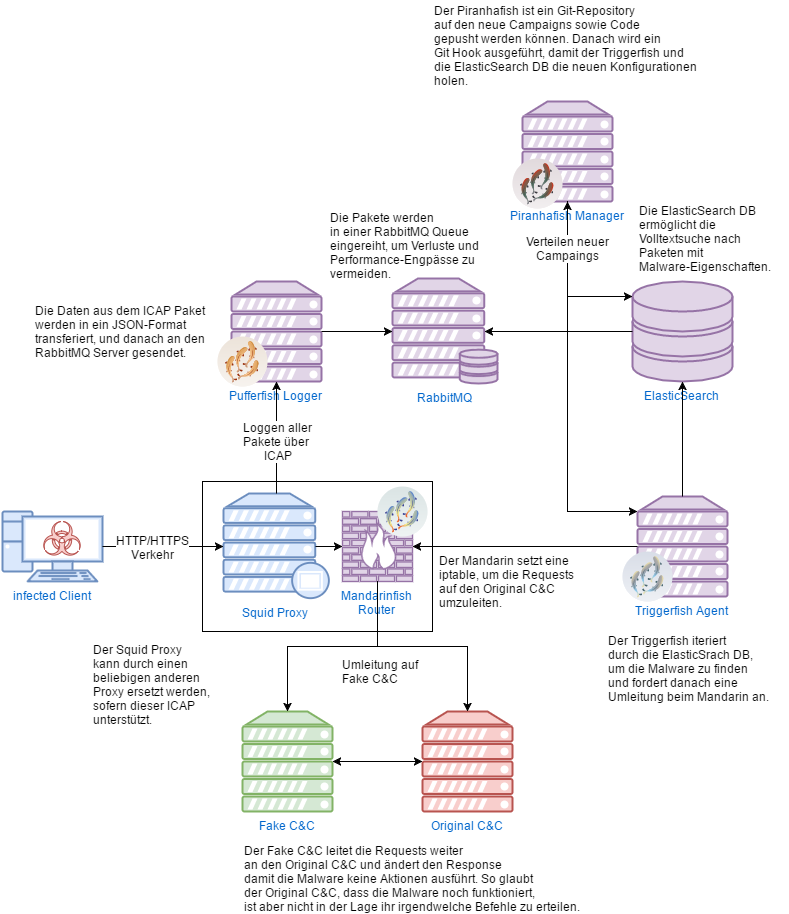
\includegraphics[width=0.85\textwidth]{img/FTS-Systemubersicht.png}
	\caption{Fish Tank Suite: Systemübersicht}
	\label{fig:Fish_Tank_Suite_Systemübersicht}
\end{figure}


\begin{figure}[H]
	\subsection{Deployment Model}
	\centering
	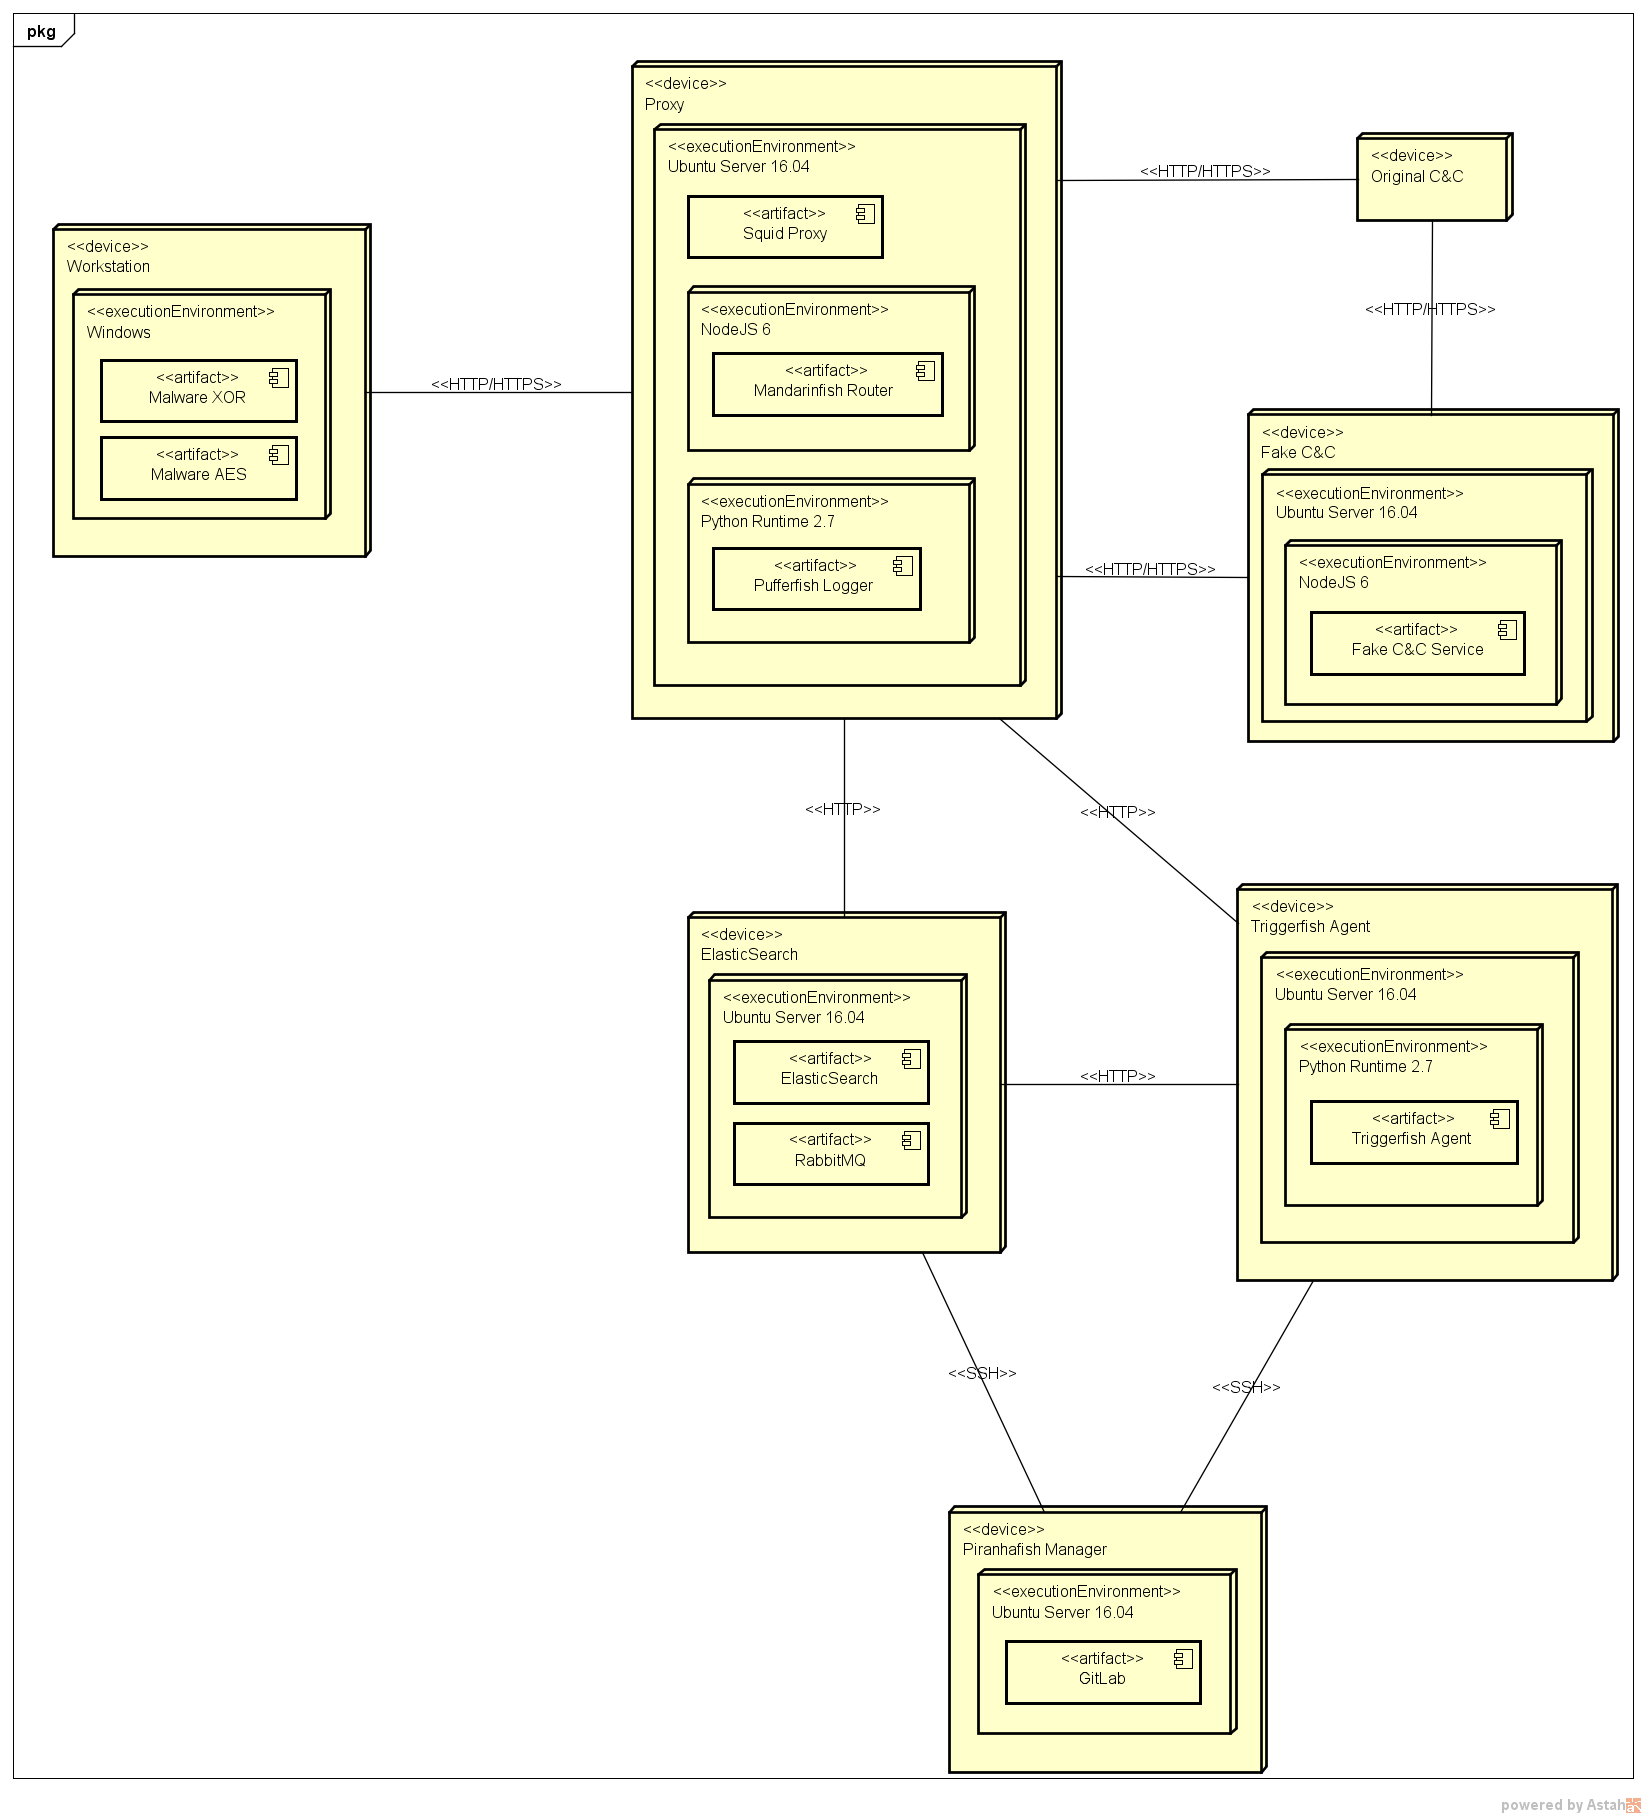
\includegraphics[width=\textwidth]{img/DeploymentDiagram.png}
	\caption{Fish Tank Suite: Deployment Model}
	\label{fig:Fish_Tank_Suite_Deployment_Model}
\end{figure}


\begin{figure}[H]
	\subsection{System Sequence Diagram}
	\centering
	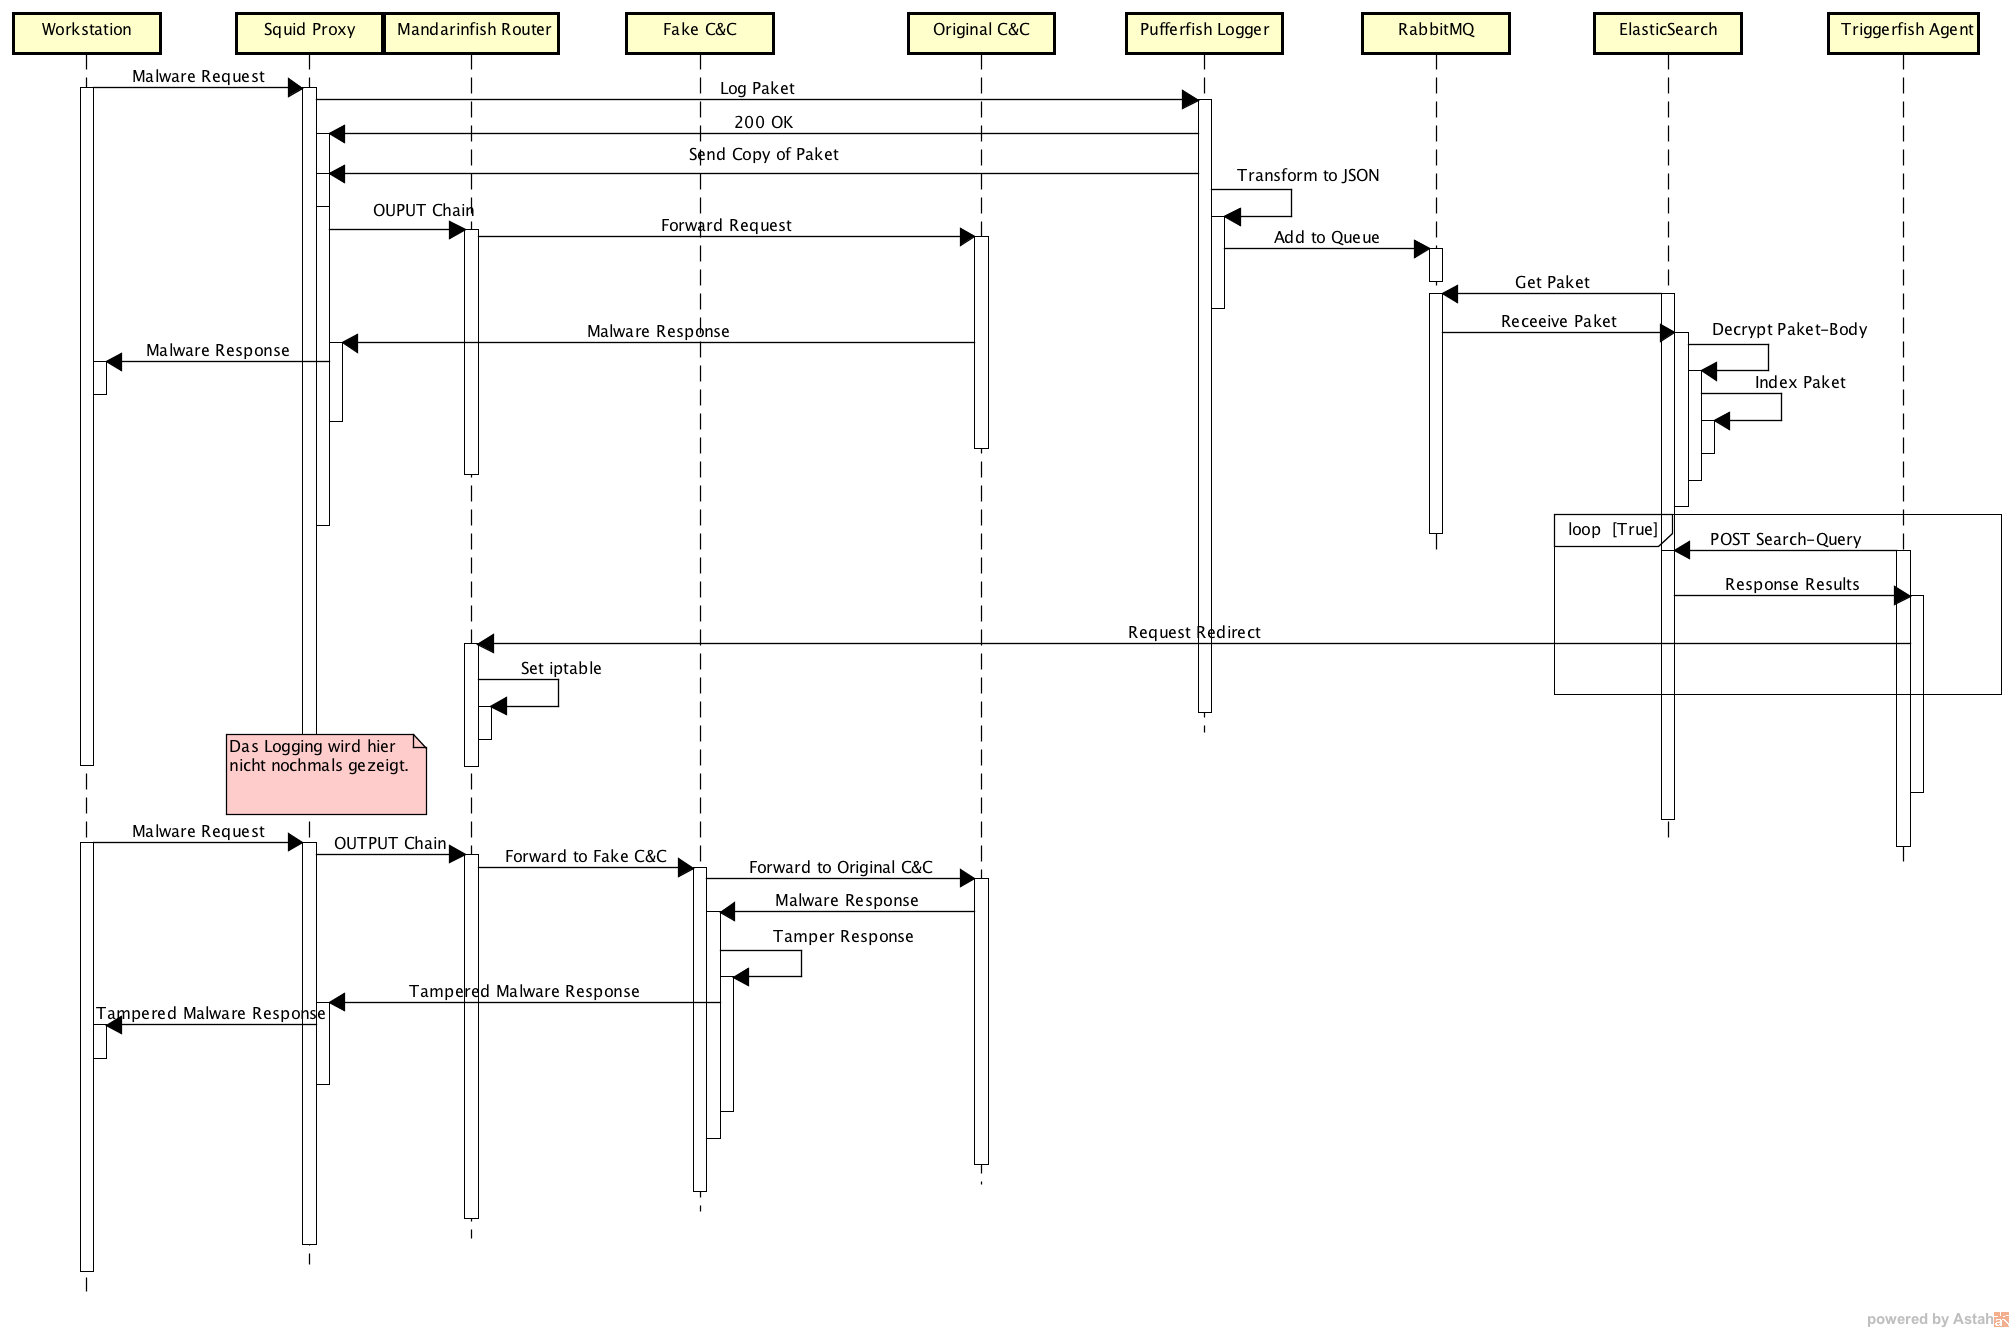
\includegraphics[width=\textwidth]{img/SequenceDiagram.png}
	\caption{Fish Tank Suite Sequence Diagram}
	\label{fig:Fish_Tank_Suite_Sequence_Diagram}
\end{figure}

%Squid Proxy
\subsection{Squid Proxy}
\label{fts:squid}
Der Squid Proxy ist die zentrale Schnittstelle, da alle HTTP Requests und Responses über ihn laufen und er entscheidet, ob gewisse Requests oder Responses geloggt werden sollen oder ob der HTTPS Verkehr von gewissen Domains nicht entschlüsselt werden soll.

\subsubsection{\gls{acl}}
Um gewisse Domains vom Entschlüsseln oder Loggen auszunehmen, kann eine \gls{acl} für die jeweilige Option (\gls{ssl} Splitting, \gls{icap} Logging) erstellt werden.

\begin{listing}[H]
\begin{fancycode}
acl icap_bypass_to_localnet dst 10.0.0.0/8
acl icap_bypass_to_localnet dst 172.16.0.0/12 
acl icap_bypass_to_localnet dst 192.168.0.0/16
\end{fancycode}
\caption{Fish Tank Suite: Squid Proxy ACL Beispiel}
\label{lst:squid-proxy-acl}
\end{listing}

\subsubsection{\gls{ssl} Splitting}
Um auch verschlüsselten Verkehr einsehen zu können, müssen alle HTTPS Verbindungen ''gebumpt'' werden, ausser man will Ausnahmen für gewisse Domains, dies wäre über eine \gls{acl} möglich.
Zusätzlich wird ein Zertifikat benötigt, welches dann an die Clients ausgeliefert wird.

\begin{listing}[H]
\begin{fancycode}
ssl_bump stare all
ssl_bump bump all
http_port 3128 ssl-bump generate-host-certificates=on dynamic_cert_mem_cache_size=4MB cert=/etc/squid/certs/myca.pem
\end{fancycode}
\caption{Fish Tank Suite: Squid Proxy SSL Bump}
\label{lst:squid-proxy-ssl-bump-config}
\end{listing}

Die Option ''generate-host-certificates'' setzt die jeweilige aufgerufene Domain als \gls{cn} für das generierte Zertifikat. 



\subsubsection{\gls{icap} Client}
Der Squid Proxy beinhaltet den \gls{icap} Client, welcher in regelmässigen Abständen den Pufferfish Logger anfragt, ob sich was an den \gls{icap} Options geändert hat und sendet jeden Request oder Response, der nicht durch eine \gls{acl} ausgenommen wurde, an den Pufferfish Logger.
Dabei müssen REQMOD und RESPMOD als einzelne Services konfiguriert sein, sehr wichtig ist das ''bypass=0'', welches das Umgehen des \gls{icap} Servers nicht erlaubt, es sei denn, es gibt eine \gls{acl} dafür.

\begin{listing}[H]
\begin{fancycode}
# Pufferfish ICAP Service
icap_service pufferfish1 reqmod_precache icap://127.0.0.1:1344/log_requests bypass=0 on-overload=wait
icap_service pufferfish2 respmod_precache icap://127.0.0.1:1344/log_responses bypass=0 on-overload=wait
\end{fancycode}
\caption{Fish Tank Suite: Squid Proxy \gls{icap} Server Config}
\label{lst:squid-proxy-icap-service}
\end{listing}


\begin{listing}[H]
\begin{fancycode}
# Adaptation Access
adaptation_access pufferfish1 deny icap_bypass_to_localnet
adaptation_access pufferfish2 deny icap_bypass_to_localnet
\end{fancycode}
\caption{Fish Tank Suite: Squid Proxy Adaptation Access Config}
\label{lst:squid-proxy-adaptation-access}
\end{listing}

Da der Pufferfish den ganzen Request oder Response benötigt, muss vom Squid Proxy auch der ganze gesendet werden und nicht bloss die Preview (einige Bytes des Requests oder Responses).

\begin{listing}[H]
\begin{fancycode}
# Disable Preview
icap_preview_enable off
\end{fancycode}
\caption{Squid Proxy Preview Konfiguration}
\label{lst:squid-proxy-preview-disable}
\end{listing}


%Squid Proxy

%Pufferfish
\subsection{Pufferfish Logger}
Der Pufferfish Logger loggt jeden Request oder Response inklusive dessen Body. Beim Prototyp V2 wurde noch darauf verzichtet die Responses zu loggen, welche nun ebenfalls geloggt werden.
Die Logs werden dabei an eine RabbitMQ gesendet, wo diese zwischengespeichert werden bis sie durch Logstash abgearbeitet werden.


\subsubsection{REQMOD}
Die Requests müssen für die Elasticsearch in ein verständliches Format gebracht werden, falls der Body mal leer sein sollte, wird ein leerer String gesetzt, damit bei der späteren Bearbeitung nicht ein Fehler bezüglich fehlendem Body auftritt.

\begin{listing}[H]
\begin{jscode}
{
  "method" : "CONNECT",
  "message": "REQMOD",
  "uri" : "hsr.ch:443",
  "headers" : {
  	 "host" : ["hsr.ch:443"],
  	 "user-agent" : ["curl"]
   },
  "body" : "",
  "level" : "INFO",
  "type" : "logstash",
  "host" : "mandarin",
  "logger_name" : "python-logstash-logger",
  "protocol_version": "HTTP/1.1",
  "path": "/home/ccproxy/Git/pufferfish-logger/__main__.py" 
}
\end{jscode}
\caption{Fish Tank Suite: REQMOD logging Beispiel}
\label{lst:pufferfish-reqmod-logging}
\end{listing}
\newpage
\subsubsection{RESPMOD}
Dasselbe beim Response, hier wird der ganze Body mitgesendet, ausser es handelt sich um einen Dateityp, der im ''Transfer-Ignore'' gesetzt ist.
\begin{listing}[H]
\begin{jscode}
 {
    "headers": {
      "date": ["Fri, 25 Nov 2016 17:31:12 GMT"],
      "content-length": ["1270"],
      "server": ["EOS (lax004/28A3)"],
      "last-modified": ["Fri, 09 Aug 2013 23:54:35 GMT"],
      "expires": ["Fri, 02 Dec 2016 17:31:12 GMT"],
      "etag": ["\"359670651\""],
      "content-type": ["text/html"],
      "accept-ranges": ["bytes"],
      "cache-control": ["max-age=604800"]
    },
    "path": "/home/ccproxy/Git/pufferfish-logger/__main__.py",
    "level": "INFO",
    "host": "mandarin",
    "logger_name": "python-logstash-logger",
    "message": "RESPMOD",
    "body": "<html>...",
    "type": "logstash",
    "tags": [],
    "status": ["HTTP/1.1","200","OK"]
}    
\end{jscode}
\caption{RESPMOD logging Beispiel}
\label{lst:pufferfish-respmod-logging}
\end{listing}
%Pufferfish

%RabbitMQ
\subsection{RabbitMQ}
Der Pufferfish erstellt beim Loggen (falls noch nicht vorhanden) einen neuen Exchange, der auf ''Durable'' gesetzt wird, damit dieser einen Neustart des RabbitMQ Servers überlebt.

Der Exchange wird als Fanout Exchange definiert, damit jede Queue, die sich mit dem Exchange verbindet, alle Messages bekommt. Routing Keys spielen keine Rolle.

\begin{figure}[H]
	\centering
	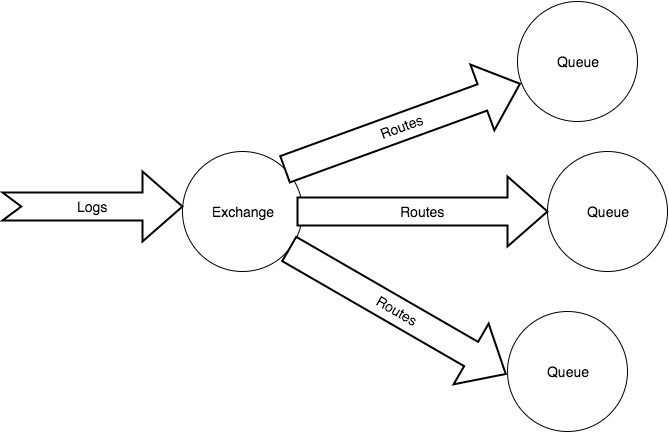
\includegraphics[width=0.8\textwidth]{img/RabbitMQ.png}
	\caption{Fish Tank Suite: Fanout Exchange}
	\label{fig:rabbitmq-fanout-exchange}
\end{figure}
%RabbitMQ

%Logstash
\subsection{Logstash}
Logstash durchläuft 3 Schritte für jede entgegengenommene Message aus der RabbitMQ.


\paragraph{Input} Als erstes nimmt Logstash die Message aus der Queue entgegen und gibt sie im Plain Format weiter an den nächsten Schritt.

\subsubsection{Filter}
Beim Filter handelt es sich nun um eine speziell für die vorhandene Malware geschriebenen Software, die verschlüsselte Payloads (XOR oder AES) entschlüsseln kann und markiert die Entschlüsselten mit Campaign Name und Cipher Art.

\newpage
\textbf{Domain Modell}
\begin{figure}[H]
	\centering
	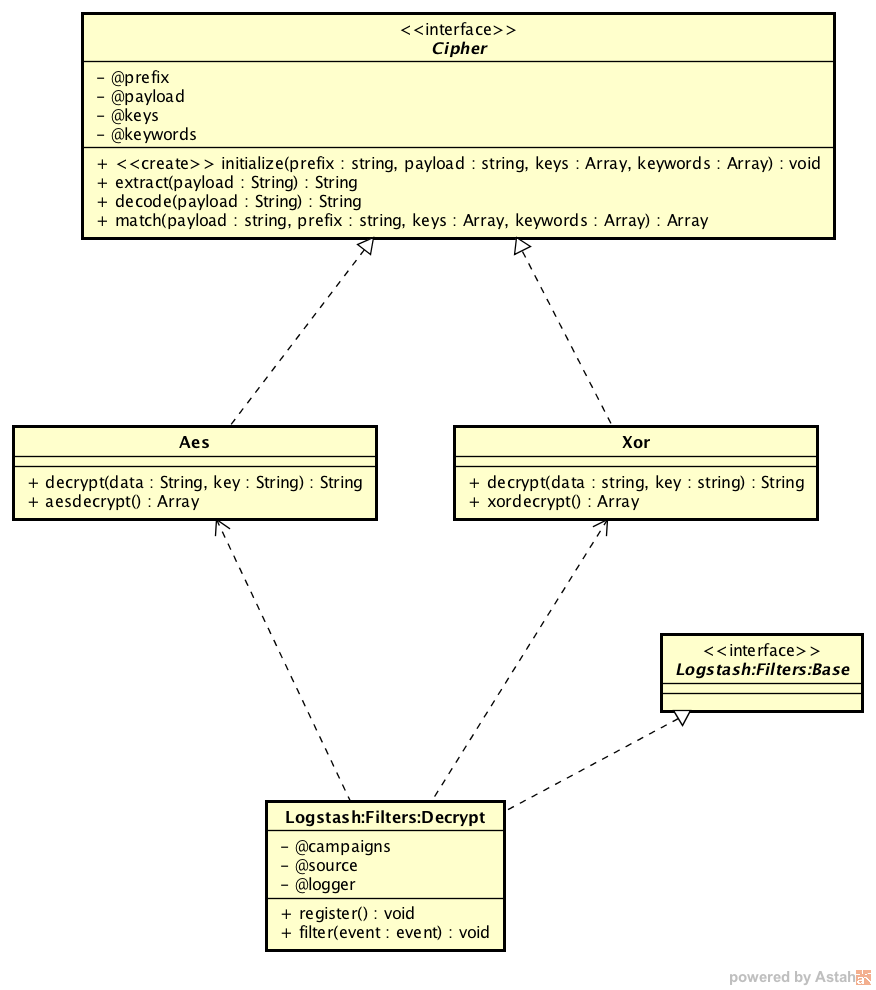
\includegraphics[width=\textwidth]{img/LogstashFilterClassDiagram}
	\caption{Fish Tank Suite: Logstash Decrypt Filter Klassendiagramm}
	\label{fig:logstash-decrypt-filter-klassendriagramm}
\end{figure}


\newpage
\textbf{Ablauf}
\begin{figure}[H]
	\centering
	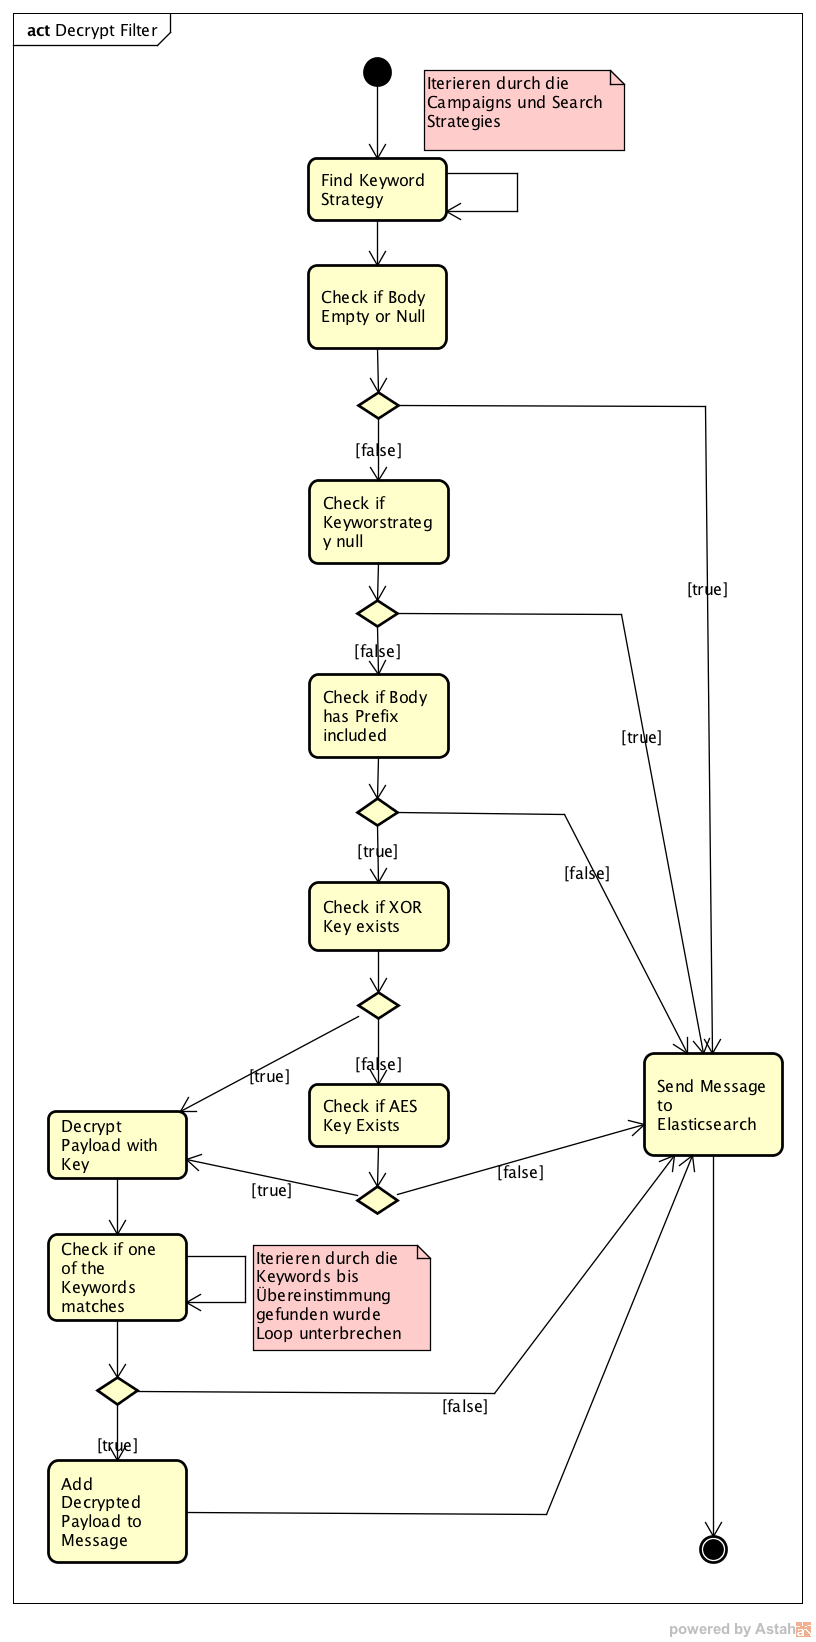
\includegraphics[width=0.60\textwidth]{img/DecryptFilterActivitiyDiagram}
	\caption{Fish Tank Suite: Logstash Decrypt Filter Ablauf}
	\label{fig:logstash-decrypt-filter-ablauf}
\end{figure}

\paragraph{Output} Zm Abschluss wird die bearbeitete Message aus der Queue in eine Elasticsearch gespeichert, dabei werden die Messages alle unter dem gleichen Index abgespeichert.

\begin{listing}[H]
\begin{fancycode}
logstash-YYYY.MM.DD
\end{fancycode}
\caption{Fish Tank Suite: Elasticsearch Index Pattern}
\label{lst:elasticsearch-index-pattern}
\end{listing}
%Logstash


%Campaign
\subsection{Campaign}
Bei der Campaign handelt es sich um die zentrale Konfiguration, um eine bekannte Malware zu erkennen.

Die Campaign bietet dabei folgende Konfigurationsmöglichkeiten:



\paragraph{name} Name der Campaign, dieser Name wird auch beim Logstash Decrypt Filter zum taggen verwendet.

\paragraph{redirectIP} IP des Fake \gls{cc}, auf welchen weitergeleitet werden soll.

\paragraph{prefix} Möglicher Prefix des Payloads, welcher nicht zum Entschlüsseln benötigt wird.

\paragraph{portRedirects} Für welche Ports ein Redirect gesetzt werden soll. Der \textit{orignalPort} ist der Port auf dem Original \gls{cc}. Der \textit{redirectPort} ist der Port vom Fake \gls{cc}.

\paragraph{SearchStrategies} Beinhaltet alle möglichen Strategien, um eine Malware zu erkennen. Für die Fish Tank Suite existieren 2 mögliche Strategien, nämlich die KeywordStrategy und die UriSequenceStrategy.

\paragraph{encryption} Die Encryption Arten, die auftreten könnten. Für die Fish Tank Suite sind das XOR oder AES und deren Schlüssel.

\begin{listing}[H]
\begin{jscode}
{
  "name": "C1",
  "redirectIp": "ip",
  "portRedirects": [
    {
      "originalPort": "port",
      "redirectPort": "port"
    },
    {
      "originalPort": "port",
      "redirectPort": "port"
    }
  ],
  "SearchStrategies": [
    {
      "name": "uri",
      "type": "UriSequenceStrategy",
      "sequence": {
        "entry": {"uri": "pattern"},
        "next": {"uri": "pattern", "timeSpan": "seconds"}
      }
    },
    {
      "name": "payload",
      "type": "KeywordStrategy",
      "prefix" : "prefix",
      "keywords": [
        "keyword"
      ]
    }
  ],
  "encryption" : {
  	"xor" : ["key"],
  	"aes" : ["key"]
  }
}
\end{jscode}
\caption{Fish Tank Suite: Campaign Beispiel mit allen Optionen}
\label{lst:campaign-json-all-options}
\end{listing}
%Campaign



\subsection{Triggerfish Agent}
Der Triggerfish Agent sucht anhand von SearchStrategies nach der Malware und setzt über den Mandarinfish einen Redirect. Die Funktionsweise der verschiedenen Strategies wird im Kapitel \ref{analyse:chapter} Abschnitt \ref{analyse:detection} beschrieben. Die Suche nach den Malwares kann parallel ausgeführt werden, was im Prototyp V2 noch nicht möglich war.

\subsubsection{Domain Model}

\begin{figure}[H]
	\centering
	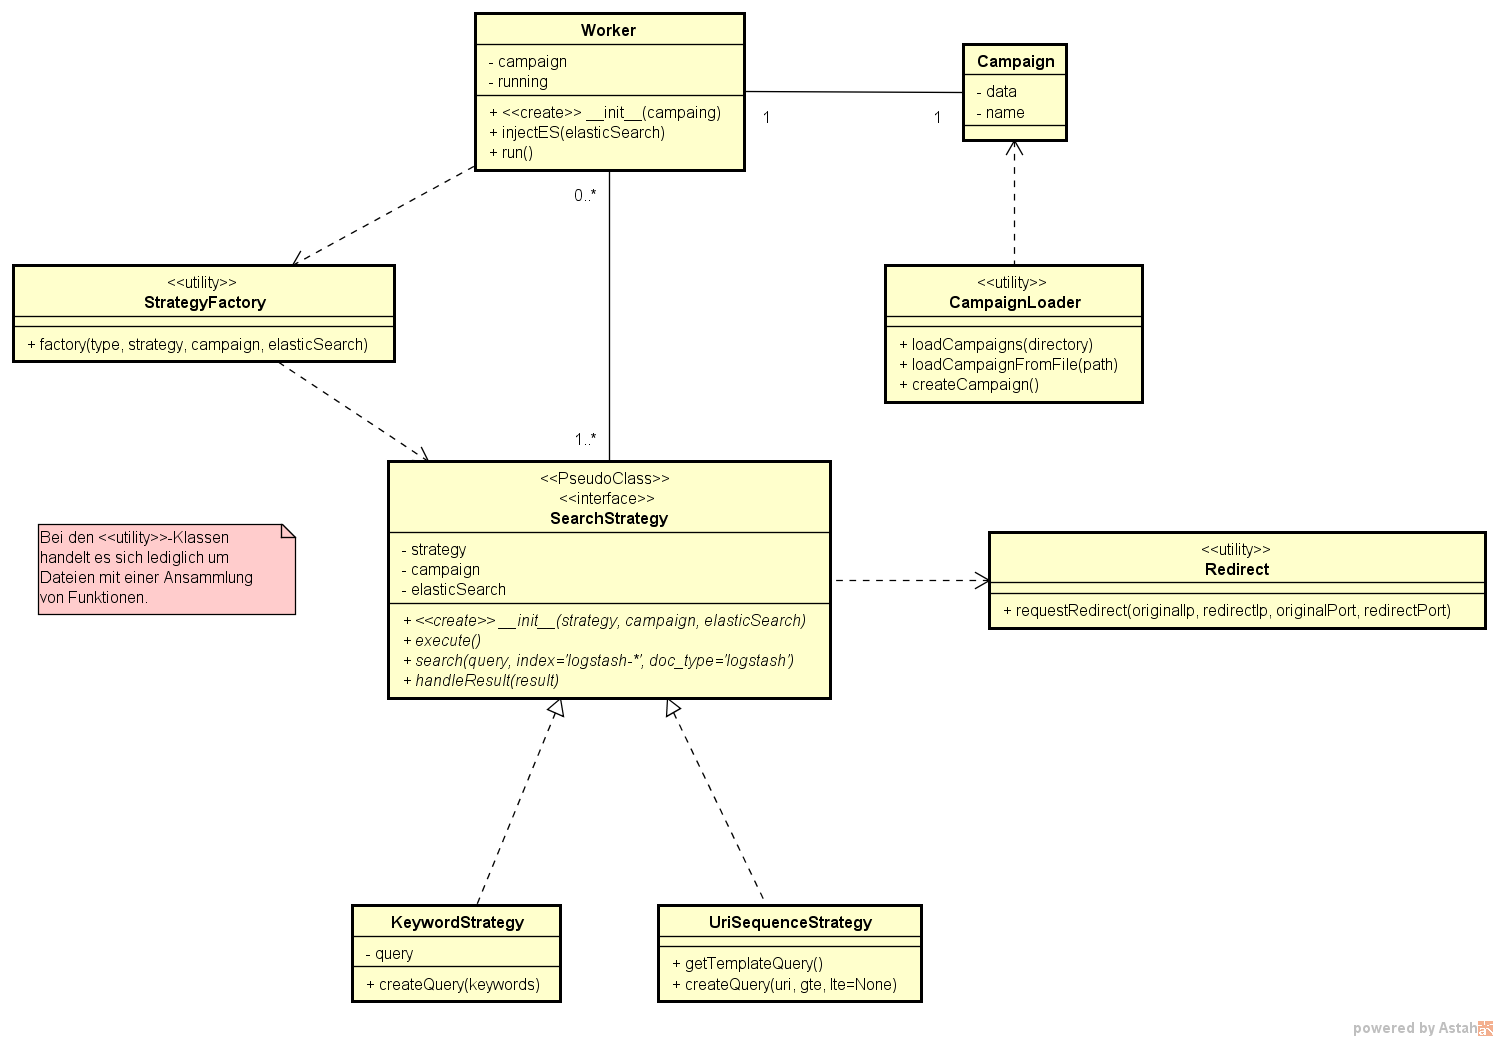
\includegraphics[width=\textwidth]{img/TriggerClassDiagram.png}
	\caption{Fish Tank Suite: Triggerfish Class Diagram}
	\label{fig:Triggerfish_Class_Diagram}
\end{figure}

\paragraph{Worker}
Der Worker implementiert die Thread-Klasse und kann deshalb mit anderen Workern parallel ausgeführt werden. Jeder Worker besitzt genau eine Campaign, die mehrere Strategies beinhalten kann.

\paragraph{Campaign}
Die Campaign kapselt die Informationen, die das Campaign-Konfigurationsfile liefert.

\paragraph{CampaignLoader}
Der CampaignLoader ist wie alle anderen Utilities keine Klasse, sondern eine Datei, die ausschliesslich Funktionen beinhaltet. Wichtig ist nur die Funktion "loadCampaigns()", welche alle JSON-Dateien lädt, die die Konfiguration einer Campaign beinhalten.

\paragraph{SearchStrategy}
Die Searchstrategy ist eine PseudoKlasse, was in anderen Sprachen, wie zum Beispiel Java, als abstrakte Klasse bezeichnet wird. Die SearchStrategy bietet einen Konstruktor, einige Hilfsfunktionen und die Funktion ''execute()'', welche die Suche nach der Malware startet.

\paragraph{StrategyFactory}
Die StrategyFactory instantiiert die konkreten Strategies.

\paragraph{Redirect}
Die Funktion ''requestRedirect()'' sendet die Informationen für einen Redirect an den Mandarinfish-Router.


\subsection{Mandarinfish Router}
Der Mandarinfish Router ist von der Funktionsweise her fast gleich wie beim Prototyp V2. Es ist nun auch möglich den Port umzuleiten, das hat den Vorteil, dass der Fake \gls{cc} nicht auf Port 80 und 443 laufen muss. Zudem ist es nun möglich mehrere Fake \gls{cc} auf dem selben Host zu betreiben. Im Prototyp V2 war es noch möglich doppelte und ungültige Iptables zu setzten. Das  wurde, wie im Activity Diagram ersichtlich, verbessert.

\subsubsection{\gls{rest} \gls{api}}

\begin{table}[H]
    \centering
	\begin{tabularx}{\textwidth}{| l | X |}
        \hline
        \textbf{Titel} & Setze Redirect \\\hline        
        \textbf{URL} & /v1/redirect \\ \hline
        \textbf{Method} & POST\\ \hline
        \textbf{Data Params} & \pbox{30cm}{\vspace{3mm} \{\\originalIp: [string], \\ redirectIp: [string],\\ originalPort: [string],\\ redirectPort: [string] \} \vspace{3mm}}\\ \hline
        \textbf{Success Repsonse} & \pbox{30cm}{\vspace{3mm} \textbf{Code:} 200 \\ \textbf{Content:} - \vspace{3mm}}\\ \hline
        \textbf{Error Response} & \pbox{30cm}{\vspace{3mm} \textbf{Code:} 400 \\ \textbf{Content:} - \\
        \textbf{Code:} 400 \\ \textbf{Content:} \{error: 'Malformed Syntax'\} \vspace{3mm}}\\ \hline
    \end{tabularx}
    \caption{Fish Tank Suite: Setze Redirect API}
\end{table}


\subsubsection{Activity Diagram}
Die Parameter der \gls{rest} \gls{api} müssen validiert werden, da Shell-Befehle ausgeführt werden, ansonsten wären Command-Injections möglich. Es dürfen auch keine doppelten oder ungültigen Iptables gesetzt werden.

\begin{figure}[H]
	\centering
	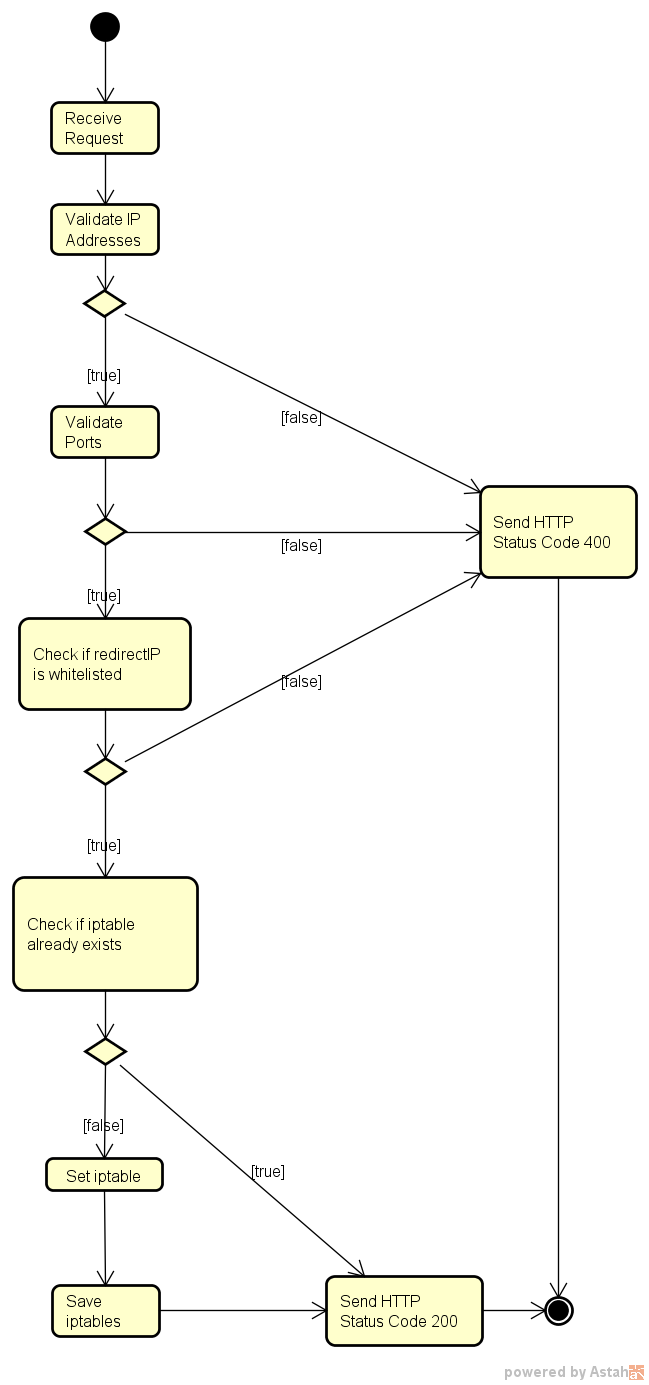
\includegraphics[width=0.5\textwidth]{img/MandarinActivityDiagram.png}
	\caption{Fish Tank Suite: Mandarin Activity Diagram}
	\label{fig:Fish_Tank_Suite_Mandarin_Activity_Diagram}
\end{figure}

\subsubsection{Iptable persistence}
Damit die Iptables nach einem Neustart des Servers noch vorhanden sind, werden die Iptables im Schritt ''Save Iptables'' in eine Datei geschrieben. Die Software ''Iptable-persistence'' stellt nach einem Neustart die Iptables wieder her.


\subsection{Piranhafish Manager}
Beim Piranhafish Manager handelt es sich um eine Gitlab\footnote{\url{https://gitlab.com}} Instanz, welche für die Handhabung der Campaigns des Triggerfish und Decrypt Filters zuständig ist.
Dabei wird über Git Hooks sichergestellt, dass alle Systeme immer auf dem neusten Stand gegenüber dem Piranhafish sind. Dazu existiert ein Campaign Git Repository, welches die Repos vom Logstash Decrypt Filter und des Triggerfishs als seine Git Submodules konfiguriert hat.
Auf den jeweiligen Zielsystemen befinden sich ebenfalls Mirrors des Campaign Git Repository, welche eigene Hooks besitzen, um die auf dem jeweiligen Host aufgeschaltete Software zu aktualisieren.

\paragraph{Piranhafish Hook} Der Prianhafish Hook pusht auf alle seine Origins, sobald der push auf das Campaign Repo beendet wurde (post-recieve).


\paragraph{Triggerfish Hook} Der Triggerfish Hook wird ausgeführt, sobald der Push vom Piranhafish beendet wurde, dabei wird auch die neuste Version des Triggerfishs gepullt.

\paragraph{Logstash Decrypt Filter Hook} Der Logstash Decrypt Filter Hook wird nach dem Push vom Piranhafish ausgeführt und pullt dabei die neuste Version des Decrypt Filters.

\subsubsection{Ablauf}

\begin{figure}[H]
	\centering
	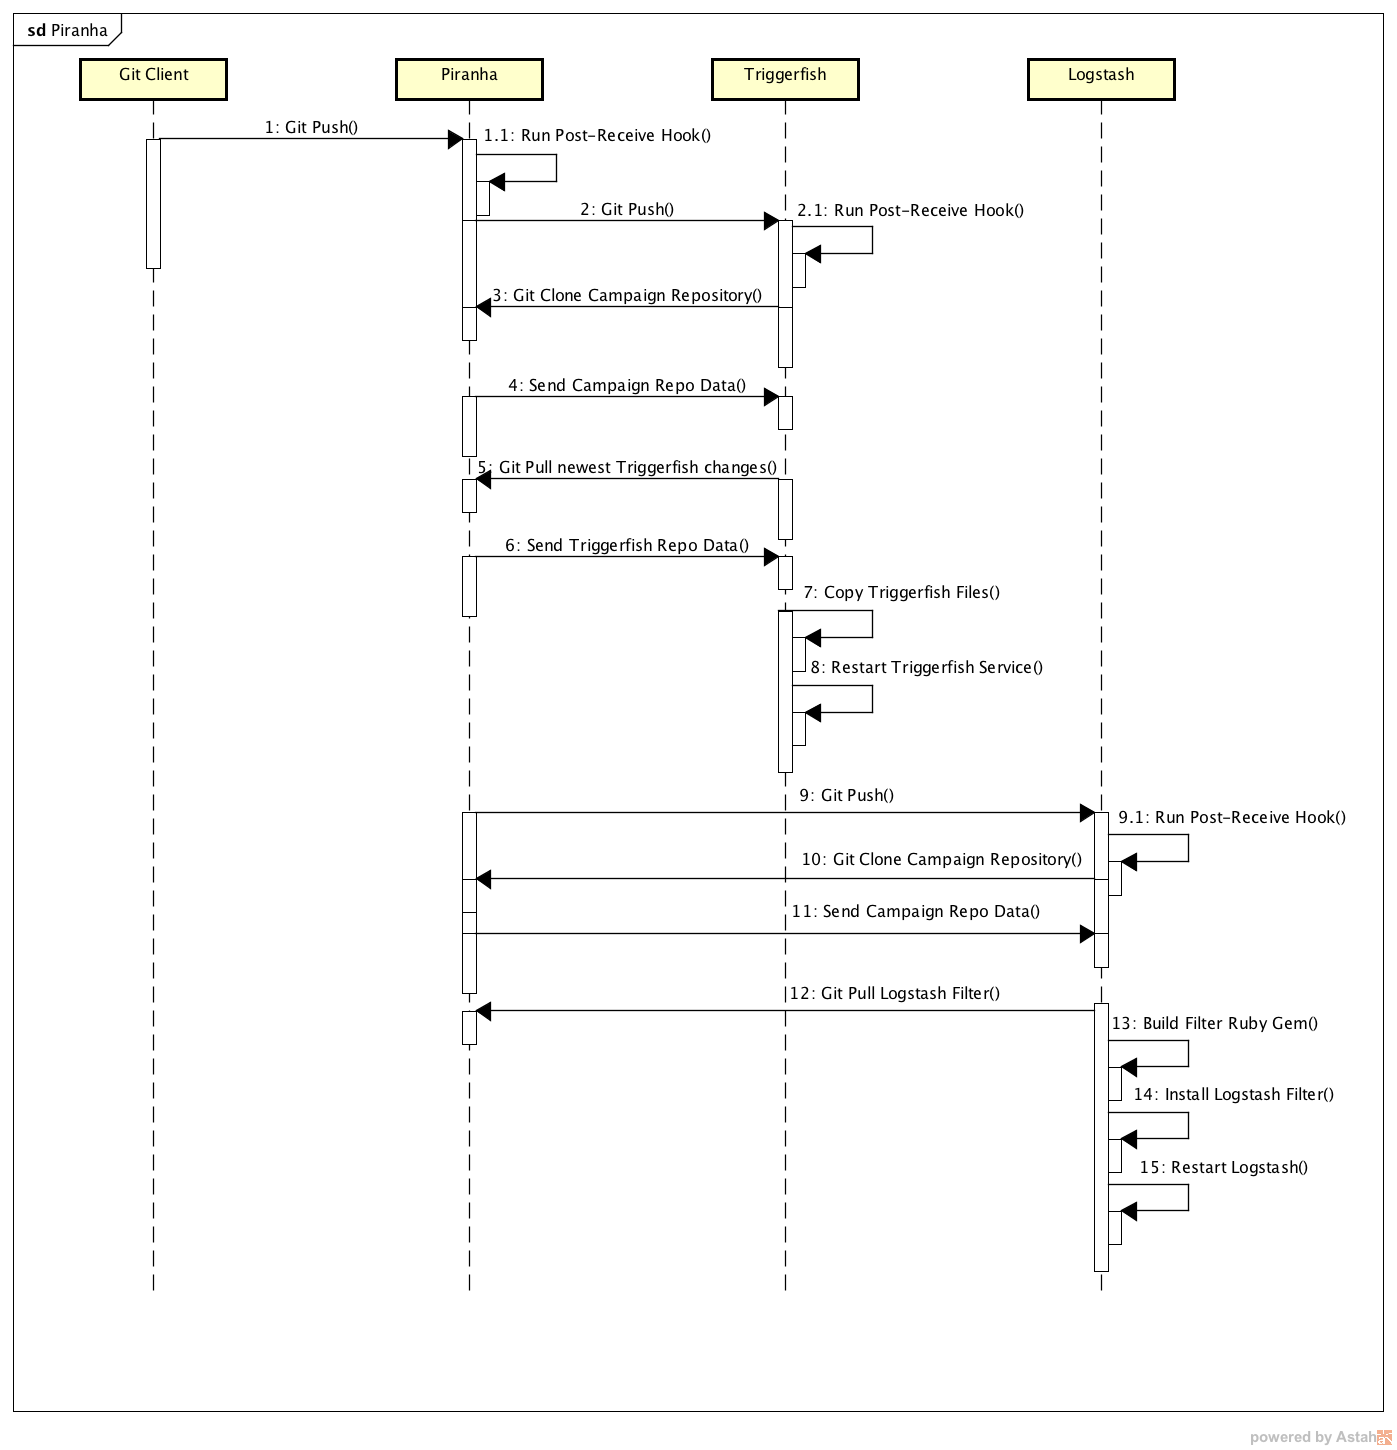
\includegraphics[width=\textwidth]{img/PiranhaSequenceDiagram.png}
	\caption{Fish Tank Suite: Piranha Git Hooks}
	\label{fig:piranha-git-hooks}
\end{figure}



\subsection{Fake Command \& Control}

Der Fake \gls{cc} wird erst aktiv, sobald der erste Request der Malware redirected wurde, dabei hört der Fake \gls{cc} nur einen Port ab und zwar für HTTP.

\begin{table}[H]
    \centering
	\begin{tabularx}{\textwidth}{| l | X |}
        \hline
        \textbf{Titel} & Request Forwarden \\\hline        
        \textbf{URL} & * \\ \hline
        \textbf{Method} & POST\\ \hline
        \textbf{Data Params} & Keine, ganzer Request wird kopiert. \\ \hline
        \textbf{Success Response} & Sende Response von Original \gls{cc} an Client zurück \\ \hline
        \textbf{Error Response} & - \\ \hline
    \end{tabularx}
    \caption{Fish Tank Suite: Request forwarding}
\end{table}

\begin{table}[H]
    \centering
	\begin{tabularx}{\textwidth}{| l | X |}
        \hline
        \textbf{Titel} & Response modifizieren \\\hline        
        \textbf{URL} & /pattern/ \\ \hline
        \textbf{Method} & POST\\ \hline
        \textbf{Data Params} & Keine, ganzer Request wird kopiert. \\ \hline
        \textbf{Success Response} & Sende modifizierten Response zurück an Client. \\ \hline
        \textbf{Error Response} & - \\ \hline
    \end{tabularx}
    \caption{Fish Tank Suite: Request forwarding}
\end{table}

\section{Testing}
In diesem Abschnitt wird die Fish Tank Suite im Detail getestet. Es wird darauf verzichtet, bereits getestete Funktionen aus der Proof of Concept Validierung nochmals zu testen.

\subsection{Testfälle}
Die Testfälle werden mit dem Pattern FTS (Fish Tank Suite) gekennzeichnet.

\begin{table}[H]
	\subsubsection{FTS-T01 Keyword Strategy}
    \centering
	\begin{tabularx}{\textwidth}{| l | p{0.6\textwidth} |}
        \hline
        \textbf{ID/Bezeichnung} & P1-T01 - Keyword Strategy\\ \hline
        \textbf{Beschreibung} &  Die Keyword Strategy versucht in verschlüsseltem Payload einen Match für ein gewisses Keyword zu finden.\\ \hline  
        \textbf{Testvoraussetzung} &  Fish Tank Suite vollständig aufgesetzt, alle Systeme aktiv , keine Iptable auf dem Mandarinfish gesetzt, Malware konfiguriert und Squid Proxy als Systemproxy hinterlegt.\\ \hline      
        \textbf{Testschritte} & 
        \begin{enumerate}
        	\item XOR oder AES Malware starten
        	\item Auf Kibana prüfen, ob Requests geloggt werden
        	\item Auf dem Mandarinfish prüfen, ob Iptable gesetzt
        	\item Fake \gls{cc} Access log für Keyword Strategy prüfen, ob Requests umgeleitet werden
        \end{enumerate} \\ \hline    
        \textbf{Erwartetes Ergebnis} &  Requests können durch den Logstash Decrypt Filter entschlüsselt und durch den Triggerfish erkannt werden. Der Triggerfish setzt dann auf dem Mandarinfish die nötige Iptable und der Fake \gls{cc} bekommt die umgeleiteten Requests.\\ \hline      
    \end{tabularx}
    \caption{Fish Tank Suite: Testfall 1}
\end{table}



\begin{table}[H]
	\subsubsection{FTS-T02 Uri Sequence Strategy}
    \centering
	\begin{tabularx}{\textwidth}{| l | p{0.6\textwidth} |}
        \hline
        \textbf{ID/Bezeichnung} & FTS-T02 - Uri Sequence Strategy\\ \hline
        \textbf{Beschreibung} &  Die Uri Sequence Strategy sucht nach einem Intervall und ein gewisses Pattern in den Ziel-Uris der Malware Requests.\\ \hline  
        \textbf{Testvoraussetzung} &  Fish Tank Suite vollständig aufgesetzt, alle Systeme aktiv , keine Iptable auf dem Mandarinfish gesetzt und Fake Malware konfiguriert und funktionsfähig.\\ \hline      
        \textbf{Testschritte} & \begin{enumerate}
        	\item Fake Malware starten und mehrere Intervalle abwarten (30s/Intervall)
        	\item Auf Mandarinfish prüfen, ob Iptable gesetzt wurde
        	\item Anhand der Konsolenausgaben vom Client prüfen, ob Request über Fake \gls{cc} umgeleitet wird.
        \end{enumerate} \\ \hline    
        \textbf{Erwartetes Ergebnis} & Der Triggerfish setzt auf dem Mandarinfish die nötige Iptable und der Fake \gls{cc} bekommt die umgeleiteten Requests.\\ \hline      
    \end{tabularx}
    \caption{Fish Tank Suite: Testfall 2}
\end{table}



\begin{table}[H]
	\subsubsection{FTS-T03 Campaign Update}
    \centering
	\begin{tabularx}{\textwidth}{| l | p{0.6\textwidth} |}
        \hline
        \textbf{ID/Bezeichnung} & FTS-T03 - Campaign Update\\ \hline
        \textbf{Beschreibung} &  Vorhandene Campaign wird angepasst und an alle nötigen Systeme verteilt.\\ \hline  
        \textbf{Testvoraussetzung} &  Fish Tank Suite vollständig aufgesetzt, alle Systeme aktiv und Push Rechte für das Campaigns Git Repository auf dem Piranhafish\\ \hline      
        \textbf{Testschritte} & \begin{enumerate}
        	\item Vorhandenes Campaign JSON anpassen
        	\item Änderungen an Piranha pushen
        	\item Auf Triggerfish prüfen, ob Änderungen übernommen wurden
        	\item Auf Elasticsearch Host prüfen, ob Campaign Änderungen übernommen wurden
        \end{enumerate} \\ \hline    
        \textbf{Erwartetes Ergebnis} & Neuste Version des Logstash Filters ist auf dem Elasticsearch Host installiert.\\ \hline      
    \end{tabularx}
    \caption{Fish Tank Suite: Testfall 3}
\end{table}

\subsection{Testprotokoll}
\subsubsection{FTS-T01 Keyword Strategy}
Zum Testen wurde folgende Konfiguration verwendet, aus Vertraulichkeitsgründen wurden jedoch die Keywords, IP's, keys und der prefix anonymisiert.
\begin{listing}[H]
\begin{jscode}
{
  "name": "C1",
  "redirectIp": "FakeCC IP",
  "portRedirects": [
    {
      "originalPort": "80",
      "redirectPort": "3000"
    }
  ],
  "SearchStrategies": [
    {
      "name": "payload",
      "prefix" : "prefix",
      "type": "KeywordStrategy",
      "keywords": [
        "keyword",
        "keyword"
      ]
    }
  ],
  "encryption" : {
   "xor" : ["key"],
   "aes" : ["key"]
  }
}
\end{jscode}
\caption{Fish Tank Suite: Keyword Search Strategy Config Beispiel}
\label{lst:keyword-strategry-config-example-protocol}
\end{listing}

Die Malware wurde gestartet und sendet verschlüsselte Requests über den System Proxy an den Original \gls{cc}.
Auf Kibana werden die Request mit Tags (Campaign Name und Cipher) markiert und können so als entschlüsselte Requests erkannt werden.

\begin{figure}[H]
	\centering
	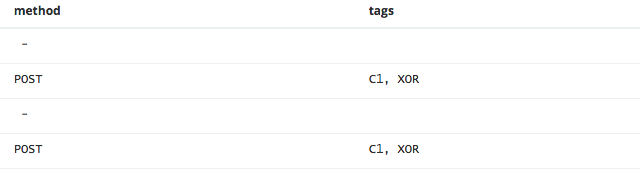
\includegraphics[width=0.7\textwidth]{img/kibana-decrypt.png}
	\caption{Fish Tank Suite: Kibana entschlüsselte Requests}
	\label{fig:kibana-decrypt}
\end{figure}


Auf dem Mandarinfish muss nun also nach relativ kurzer Zeit eine Iptable gesetzt worden sein, welche die Original \gls{cc} IP und Destination Port auf die Fake \gls{cc} IP und deren Destination Port umleitet.

\begin{listing}[H]
\begin{fancycode}
Chain PREROUTING (policy ACCEPT)
target     prot opt source               destination         

Chain INPUT (policy ACCEPT)
target     prot opt source               destination         

Chain OUTPUT (policy ACCEPT)
target     prot opt source               destination         
DNAT       tcp  --  anywhere             [OriginalCC IP]  tcp dpt:http to:[FakeCC IP]:3000

Chain POSTROUTING (policy ACCEPT)
target     prot opt source               destination 
\end{fancycode}
\caption{Fish Tank Suite: Mandarin Iptables}
\label{lst:mandarin-http-Iptable}
\end{listing}

Ebenfalls sollten nun auf dem Fake \gls{cc} die umgeleiteten Requests in seinem Log auftauchen. Die Malware sendet weiter Requests ohne zu merken, dass die Requests über den Fake \gls{cc} umgeleitet werden.
Im Access Log können die gesendeten Responses des Original \gls{cc} (die nicht modifizierten) und die Paths der Requests, die vom Client gesendet wurde, eingesehen werden.

\begin{listing}[H]
\begin{fancycode}
[2016-12-11 08:03:27.457] [INFO] fakecc - original CC Response to Client
[2016-12-11 08:03:37.678] [INFO] fakecc - path
[2016-12-11 08:03:37.769] [INFO] fakecc - original CC Response to Client
[2016-12-11 08:03:47.704] [INFO] fakecc - path
[2016-12-11 08:03:47.790] [INFO] fakecc - original CC Response to Client
\end{fancycode}
\caption{Fish Tank Suite: Fake \gls{cc} Access log}
\label{lst:fake-cc-access-log}
\end{listing}



\subsubsection{FTS-T02 Uri Sequence Strategy}
Nachfolgende Konfiguration wurde zur Erkennung einer selbst entwickelten Malware verwendet. Diese Malware unterstützt HTTPS und wird auf einen eigenen Fake \gls{cc} umgeleitet.
\begin{listing}[H]
\begin{jscode}
{
  "name": "C2",
  "redirectIp": "fakeCC-IP",
  "portRedirects": [
    {
      "originalPort": "443",
      "redirectPort": "4000"
    }
  ],
  "SearchStrategies": [
    {
      "name": "register",
      "type": "UriSequenceStrategy",
      "sequence": {
        "entry": {"uri": "register"},
        "next": {"uri": "count", "timeSpan": "30s"}
      }
    }
  ]
}
\end{jscode}
\caption{Fish Tank Suite: URI Sequence Strategy Config Beispiel}
\label{lst:uri-sequence-strategy-configuration-example-protcol}
\end{listing}


Die Fake Malware wurde gestartet und sendet nach einem ersten Register alle 30 Sekunden einen weiteren Request. Der Intervall und die Ziel-Uris \textit{register} und \textit{count} sollen nun durch den Triggerfish erkannt werden.

Sobald sie erkannt werden, wird eine Iptable gesetzt, die den HTTPS Verkehr auf den Port 4000 des Fake \gls{cc} Hosts umleitet.

\begin{listing}[H]
\begin{fancycode}
Chain PREROUTING (policy ACCEPT)
target     prot opt source               destination         

Chain INPUT (policy ACCEPT)
target     prot opt source               destination         

Chain OUTPUT (policy ACCEPT)
target     prot opt source               destination         
DNAT       tcp  --  anywhere             [OriginalCC IP]  tcp dpt:https to:[FakeCC IP]:4000

Chain POSTROUTING (policy ACCEPT)
target     prot opt source               destination  
\end{fancycode}
\caption{Fish Tank Suite: Mandarin Iptables}
\label{lst:mandarin-https-Iptable}
\end{listing}

Sobald die Iptable gesetzt ist werden alle Repsonses, die nicht an die URI \textit{register} gehen, durch den Text ''This is not from the Original Server'' ersetzt. Dieser Text wird durch den Fake \gls{cc} gesetzt.

\begin{listing}[H]
\begin{fancycode}
send: Mjc2NzI1ZDItYzZlMy00ZjQ1LWEzY2ItOGM1NzBhNmZhNzk5
path: /v1/register
received: ODc0ZjdmZDYtNjBjOC00ODY0LWIyMWQtZmY5YjdiMTc0MmVk
send: MmQ1NzkxYzUtZmU2ZS00ZGFkLTlmOTUtZTkwMzI4MWQ5NzZh
path: /v1/count
received: YWMxZDY1ZWYtMWJlNC00N2M3LTk0YWEtN2I5Yjc3NzgwNjgx
send: NTdhM2UwZmMtZWRkZC00MzZkLTlhNzMtMzA0Y2Y2OTI1MGQz
path: /v1/count
received: This is not from the Original Server
send: NDE2YWM0ODItYzBmYS00OTg1LThkZDMtMzE4YjkwZmI5ZmRi
\end{fancycode}
\caption{Fish Tank Suite: Client Log}
\label{lst:uri-client-log}
\end{listing}


\subsubsection{FTS-T03 Campaign Update}
Das Ändern einer vorhandenen Campaign kann wichtig werden, wenn neue Erkenntnisse zu einer Malware bestehen (z.B. neuer Key oder neues Keyword, nach dem geprüft werden soll).
Zusätzlich werden die neusten Änderungen vom Logstash Decrypt Filter und vom Triggerfish übernommen.

Falls der Decrypt Filter sich geändert hat und eine neue Release Version verfügbar ist (falls die installierte Version auf Elasticsearch gleich der Version vom Logstash Decrypt Filter Repository ist, wird der Filter nicht installiert), muss die Versionsnummer unter \textit{s.version} in der \textit{Gemspec} Datei angepasst werden.
Die Änderungen am Logstash Filter Decrypt müssen nun auf den Piranha Host publiziert werden, damit das Campaigns Repository über einen Git Hook die neusten Änderungen holen kann.

\begin{listing}[H]
\begin{rubycode}
Gem::Specification.new do |s|
  s.name = 'logstash-filter-decrypt'
  s.version = '0.0.2'
\end{rubycode}
\caption{Fish Tank Suite: Logstash Filter Decrypt Version}
\label{lst:logstash-filter-decrypt-version}
\end{listing}

Sobald ein neuer Push auf das Campaigns Repository stattfindet, wird der Hook ausgeführt und die neue Version des Filters installiert.

\begin{listing}[H]
\begin{fancycode}
git commit --allow-empty -m "Trigger Hook"
\end{fancycode}
\caption{Fish Tank Suite: Leerer Commit für Campaigns Repository}
\label{lst:empty-commit-campaigns}
\end{listing}

Beim nächsten push des Campaigns Repository werden alle Hooks ausgeführt und die neuere Version des Decrypt Filter auf Elasticsearch installiert.

\begin{listing}[H]
\begin{fancycode}
Counting objects: 1, done.
Writing objects: 100% (1/1), 190 bytes | 0 bytes/s, done.
Total 1 (delta 0), reused 0 (delta 0)
remote: remote: From /home/ccproxy/Git/campaigns        
remote: remote:  * branch            master     -> FETCH_HEAD        
remote: remote:    74e77d4..e0831a9  master     -> origin/master        
remote: remote: Updating 74e77d4..e0831a9        
remote: remote: Fast-forward        
remote: remote: From piranha:ccproxy/triggerfish-agent        
remote: remote:  * branch            master     -> FETCH_HEAD        
remote: remote: Already up-to-date.        
remote: To ccproxy@trigger:Git/campaigns.git
remote:    74e77d4..e0831a9  master -> master
remote:    532bd58..74e77d4  elasticsearch/master -> elasticsearch/master
remote:    532bd58..74e77d4  triggerfish/master -> triggerfish/master
remote: remote: From /home/ccproxy/Git/campaigns        
remote: remote:  * branch            master     -> FETCH_HEAD        
remote: remote:    74e77d4..e0831a9  master     -> origin/master        
remote: remote: Updating 74e77d4..e0831a9        
remote: remote: Fast-forward        
remote: remote: From prianha:ccproxy/logstash-filter-decrypt        
remote: remote:  * branch            master     -> FETCH_HEAD        
remote: remote: Already up-to-date.        
remote: remote:   Successfully built RubyGem        
remote: remote:   Name: logstash-filter-decrypt        
remote: remote:   Version: 0.0.2        
remote: remote:   File: logstash-filter-decrypt-0.0.2.gem        
remote: remote: Validating /home/ccproxy/campaigns/
logstash-filter-decrypt/logstash-filter-decrypt-0.0.2.gem        
remote: remote: Installing logstash-filter-decrypt        
remote: remote: Installation successful               
remote: To elasticsearch:Git/campaigns.git
remote:    74e77d4..e0831a9  master -> master
remote:    532bd58..74e77d4  elasticsearch/master -> elasticsearch/master
remote:    74e77d4..e0831a9  triggerfish/master -> triggerfish/master
To git@piranha.hacking-lab.com:ccproxy/campaigns.git
   74e77d4..e0831a9  master -> master
\end{fancycode}
\caption{Fish Tank Suite: Git Push Log}
\label{lst:piranha-git-push-log}
\end{listing}

Auf dem Elasticsearch Host ist nun die neuste Version des Logstash Filters installiert. Beim Triggerfish ist die Versionierung kein Problem, da immer alle Dateien überschrieben werden.

\begin{listing}[H]
\begin{fancycode}
sudo /usr/share/logstash/bin/logstash-plugin list --verbose logstash-filter-decrypt logstash-filter-decrypt (0.0.2)
\end{fancycode}
\caption{Fish Tank Suite: Logstash Filter Version}
\label{lst:logstash-filter-version}
\end{listing}


\subsection{Performance}
Um einen Einblick zu bekommen, wie performant die Fish Tank Suite Lösung ist, wurden HTTP Performance Tests durchgeführt, welche 150 Benutzer simulieren. Diese Benutzer greifen dabei auf eine Auswahl der Top 25 Wikipedia Artikel zu. Diese Requests sollen dabei über den Proxy geleitet werden.
Zusätzlich zu den 150 Benutzern wird eine Malware gestartet (Keyword Strategy).
Für die nachfolgenden Performance Tests wurde locust\cite{locust}\footnote{\url{http://locust.io/}} verwendet

Bei der Simulation sind dabei folgende Indikatoren wichtig:
\paragraph{Zeit bis Message aus der Queue} Falls nun die Queue mit Request überhäuft wird und dazwischen einzelne Requests durch Logstash entschlüsselt werden sollen, kann die Abarbeitung der Queue länger dauern als geplant.
\paragraph{Zeit bis zur Erkennung der Malware} Sobald die Message in der Elasticsearch gespeichert ist, braucht der Triggerfish einen Moment, bis er die zutreffenden Messages findet und eine Iptable auf dem Mandarinfish setzt.
\paragraph{Zeit von Erkennung bis Abwehr} Dies beinhaltet die beiden oben genannten Indikatoren und soll einen möglichst realitätsnahen Wert darstellen, wie lange es dauert, eine Malware zu entdecken und Abwehrmassnahmen einzuleiten.

\subsubsection{Logging}
Der Pufferfish loggt alles direkt in die RabbitMQ, muss allerdings von allen Requests den Body lesen, was ein blockender Aufruf ist.
Somit wird der Pufferfish auch zum Flaschenhals der Software. Wenn nicht geloggt wird, kann auch nicht entschlüsselt werden.


\textbf{HTTP Performance Vergleich zwischen ohne Proxy und mit Proxy:}
\begin{figure}[H]
	\centering
	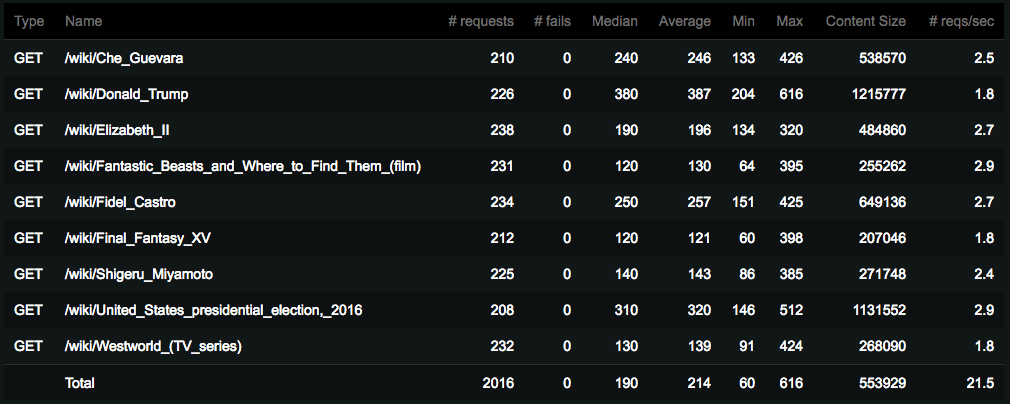
\includegraphics[width=\textwidth]{img/http-performance-no-proxy}
	\caption{Fish Tank Suite: HTTP Performance ohne Proxy}
	\label{fig:http-performance-ohne-proxy}
\end{figure}

\begin{figure}[H]
	\centering
	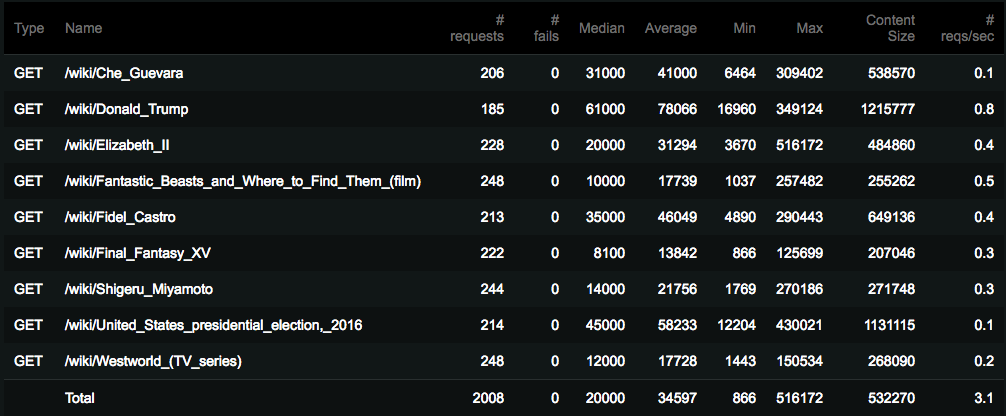
\includegraphics[width=\textwidth]{img/http-performance-proxy}
	\caption{Fish Tank Suite: HTTP Performance mit Proxy}
	\label{fig:http-performance-mit-proxy}
\end{figure}

Es gibt eine Performance Verschlechterung, wenn der ganze Traffic über den Proxy geht.
Besserung könnte hier womöglich noch ein Ausklammern der ''Known Goods'' bringen, damit nicht alles geloggt wird, sondern nur die Requests, die interessant sein könnten.

\subsubsection{Entschlüsseln}
Entschlüsselt wird auf dem Elasticsearch Host, wo der Logstash Decrypt Filter die Messages aus der RabbitMQ entgegennimmt.
Hier kann es zu Zeitverzögerungen kommen, falls eine Message aus der Queue länger benötigt und dadurch die nachfolgenden Messages stoppt.
Logstash kann allerdings gut skaliert werden, wodurch die Performance verbessert werden kann.

\textbf{Performance Logstash}
Für diesen Test wurde zusätzlich zu den 150 Benutzern eine Malware gestartet, um die Performance des Entschlüsselns mit viel nebenläufigem Verkehr beobachten zu können.


Durch den nebenläufigen Verkehr kann es zu Lastspitzen kommen, aber wie man beim Logging bereits gesehen hat, können im Durchschnitt ca. 3 Requests pro Sekunde durch den Proxy abgearbeitet werden, wodurch keine zu grosse Lastspitzen entstehen.


\begin{figure}[H]
	\centering
	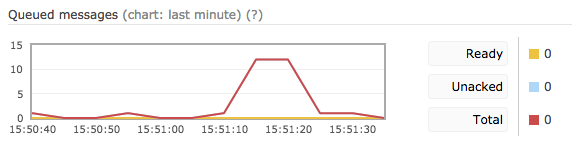
\includegraphics[width=0.7\textwidth]{img/rabbitmq-performance}
	\caption{Fish Tank Suite: RabbitMQ Lastspitzen}
	\label{fig:rabbitmq-lastspitze}
\end{figure}


Das Entschlüsseln selbst wird daher nicht allzu sehr verzögert (Event Timestamp ist der Zeitpunkt, wo die Message an die Queue gesendet wurde).
Die Entschlüsselung benötigt bloss einige Millisekunden, aber der Event kam 1 Sekunde verspätet an die Reihe.
\begin{listing}[H]
\begin{fancycode}
[2016-12-12T15:52:03,429][INFO ][logstash.filters.decrypt ] Decrypt Body
[2016-12-12T15:52:03,443][INFO ][logstash.filters.decrypt ] Event after filter {:event=>2016-12-12T14:52:02.942Z mandarin REQMOD}
\end{fancycode}
\caption{Fish Tank Suite: Logstash Log Decrypt Beispiel}
\label{lst:logstash-decrypt-filter-log}
\end{listing}

Ein Performance Engpass existiert bei der Entschlüsselung nicht, und die Möglichkeit, einen RabbitMQ Cluster und mehrere Logstash Consumers zu installieren, existiert immer.


\subsubsection{Abwehr}
Bei der Abwehr muss in möglichst kurzem Zeitraum eine Iptable gesetzt werden, um die Malware auf den Fake \gls{cc} Server umzuleiten.

Bei diesem Test wurde ebenfalls die Malware mit 150 Benutzern zusammen verwendet. Kurz nachdem die Malware gestartet wurde, wird auf dem Mandarinfish die Iptable gesetzt

\begin{listing}[H]
\begin{fancycode}
Validating IP Addresses
IP: 212.254.246.109 is v4
IP: 192.168.200.125 is v4
Validating Ports
All Port OK
Checking if redirect IP is whitelisted
IP: 192.168.200.125is in subnet: 192.168.200.0/24
is Host Adress
Check if Iptable already exists
Iptable doesnt exist
\end{fancycode}
\caption{Fish Tank Suite: Mandarinfish Iptable setzen}
\label{lst:mandarinfish-Iptable-setzen}
\end{listing}

Die umgeleiteten Requests werden auch wieder über den Fake \gls{cc} Server geleitet.

Die Abwehr und Umleitung der Requests funktioniert auch mit 150 Benutzern, die ebenfalls den Proxy verwenden.


\subsection{Zusammenfassung}
Die Fish Tank Suite hält den Datenverkehr von 150 Benutzern und mehr aus, die Geschwindigkeit lässt jedoch merklich nach.
Um die letzten Flaschenhälse zu entfernen, müsste der Pufferfish performanter werden, da aber der ganze Inhalt der Requests oder Responses gelesen werden muss, gibt es nicht viele Optimierungsmöglichkeiten.

